\documentclass[10pt]{beamer}
\usetheme{Warsaw}
\usefonttheme[onlymath]{serif} 
\setbeamercovered{invisible}
\beamerdefaultoverlayspecification{<+->}

\usepackage[utf8]{inputenc}
\usepackage[english]{babel}
\usepackage[T1]{fontenc}
\usepackage{lmodern,amsmath,booktabs,setspace,mathtools}

\title{Classification via Local Search}
\subtitle{Algorithm Design}
\author[J. Kleinberg, E. Tardos]{Jon Kleinberg, \'{E}va Tardos}
\institute{CS 210 Report \\ J Franco Ray}
\date{\today}

\begin{document}

\begin{frame}
	\maketitle
\end{frame}

\begin{frame}[noframenumbering]{Outline}
	\tableofcontents
\end{frame}

\section{Network Flow}
\subsection{Definition}
\begin{frame}{Network Flow}{}
	\begin{figure}[H]
		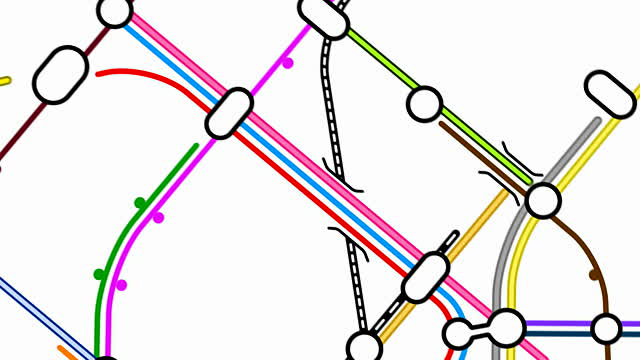
\includegraphics[width=.4\textwidth]{transport}
	\end{figure}
	\textit{Motivation}: Transportation networks carry some soft of traffic whose nodes act as 'switches' passing traffic between edges.
	\begin{itemize}
		\item<1-> capacities on the edges (how much they can carry?)
		\item<1-> source nodes (of traffic)
		\item<1-> sink nodes (destination), absorbs traffic
		\item<1-> the traffic itself
	\end{itemize}
\end{frame}

\begin{frame}{Network Flow}{}
	\begin{figure}[H]
		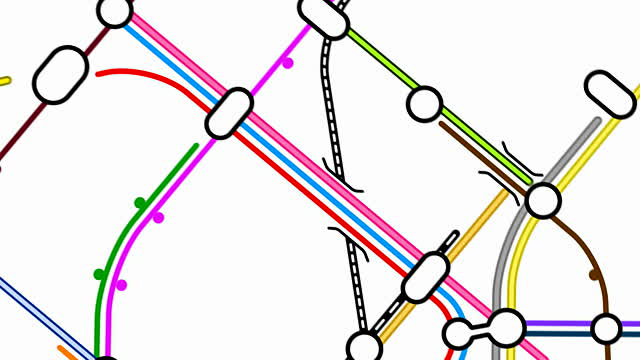
\includegraphics[width=.4\textwidth]{transport}
	\end{figure}
	\textit{Motivation}: Transportation networks carry some soft of traffic whose nodes act as 'switches' passing traffic between edges.
	\begin{itemize}
		\item<1-> capacities on the edges (how much they can carry?)
		\item<1-> source nodes (of traffic)
		\item<1-> sink nodes (destination), absorbs traffic
		\item<1-> the traffic itself
	\end{itemize}
	\textit{Question}: How much traffic can a network handle?
\end{frame}

\begin{frame}{Network Flow}
	\begin{figure}
		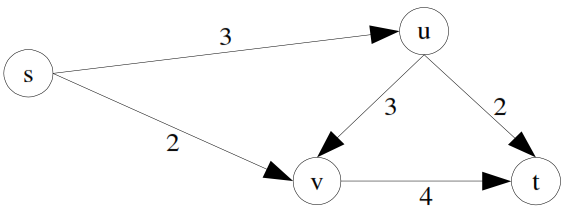
\includegraphics[width=.7\textwidth]{network}
	\end{figure}
	A flow network is a directed graph $G = (V, E)$:
	\begin{itemize}
		\item<1-> $c_e$ - capacity of the edge, nonnegative
		\item<1-> $s$ - single source node
		\item<1-> $t$ - single sink node
		\item<1-> internal nodes (traffic junctions)
	\end{itemize}
\end{frame}

%TODO: image example

\begin{frame}{Network Flow}
	\begin{figure}
		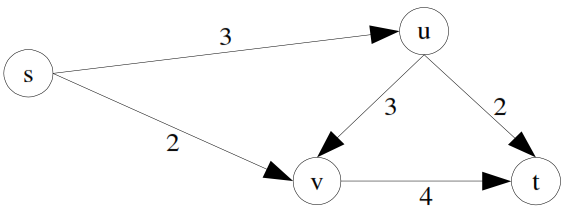
\includegraphics[width=.7\textwidth]{network}
	\end{figure}
	Some assumptions:
	\begin{itemize}
		\item<1-> no edge enters $s$ and no edge leaves $t$
		\item<1-> at least one edge incident to each node
		\item<1-> all capacities are integers 
	\end{itemize}
\end{frame}

\begin{frame}{Defining flow}
	\begin{figure}
		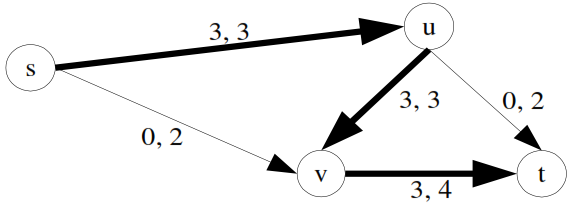
\includegraphics[width=.7\textwidth]{flow}
	\end{figure}
	A network flow is a function $f: E \rightarrow \mathbb{R}^{+}$ that represents the amount of flow on an edge.
	\begin{itemize}
		\item For each $e \in E$, $0 \leq f(e) \leq c_e$
		\item For each node $v$ other than $s, t$, $$\sum_{e\: \text{into}\:v} f(e) = \sum_{e\:\text{out of}\:v} f(e)$$
		\item $v(f)$ is the amount of flow generated at the source
	\end{itemize}
\end{frame}

\subsection{Maximum Flow Problem}
\begin{frame}{Maximum Flow Problem}
	\begin{block}{Maximum Flow Problem}
		Given a flow network, find a flow of maximum possible value.
	\end{block}
	Suppose we divide the nodes of the graph into two sets, $A$ and $B$, so that $s \in A$ and $t \in B$.
	\begin{itemize}
		\item Any flow from $s$ to $t$ must cross from $A$ to $B$ at some point and use up some of the edges from $A$ to $B$.
		\item The capacity of the cut: $c(A, B) = \sum_{e \:\text{out of}\:A}c_e$.
		\item $v(f) \leq c(A, B)$
		\item The optimal cut(s) can be solved using \textit{Ford-Fulkerson} algorithm: max flow equals min cut
	\end{itemize}
\end{frame}

\begin{frame}{Example}
	\begin{figure}
		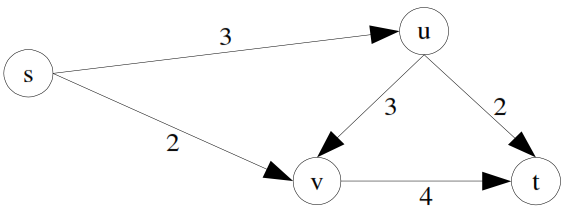
\includegraphics[width=.8\textwidth]{network}
	\end{figure}
	\begin{figure}
		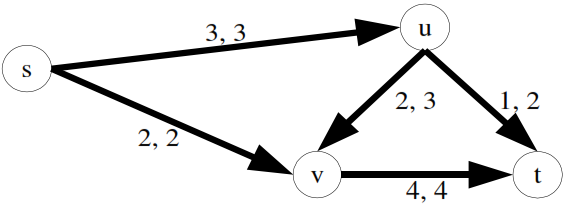
\includegraphics[width=.8\textwidth]{opt}
	\end{figure}
\end{frame}

\subsection{Image Segmentation}
\begin{frame}{Image Segmentation}
	\begin{figure}
		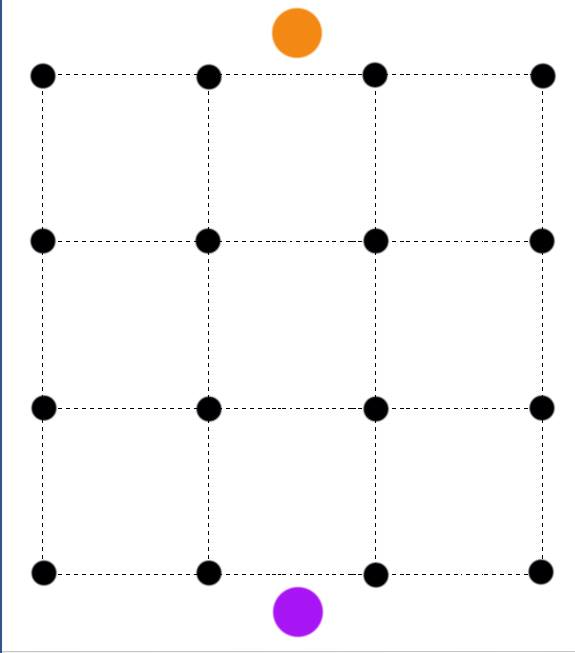
\includegraphics[width=.3\textwidth]{segment}
	\end{figure}
	We wish to label each pixel in an image as FG/BG pixel.
	\begin{itemize} 
		\item<1-> $a_i,b_i \geq 0$: likelihood that $i$ belongs to FG/BG
		\item<1-> $p_{ij} \geq 0$: separation penalty for classifying $i$ and $j$ differently
	\end{itemize}
\end{frame}

\begin{frame}{Image Segmentation}
	\begin{figure}
		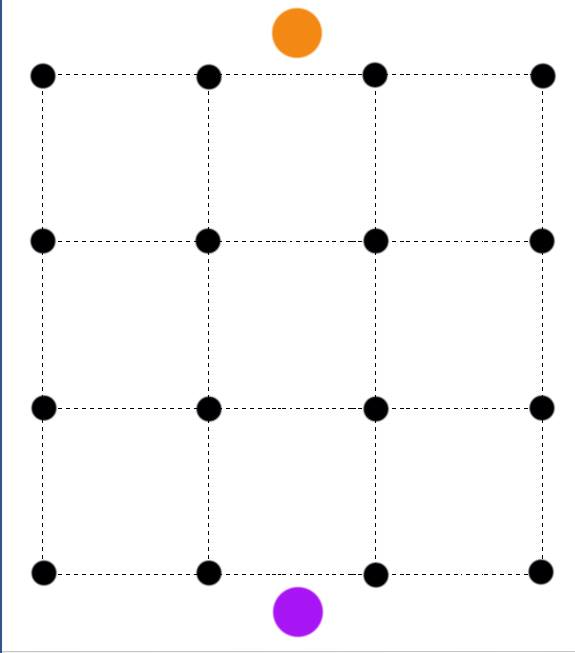
\includegraphics[width=.3\textwidth]{segment}
	\end{figure}
	\begin{block}<1->{Segmentation Problem}
		Find a partition of the set of pixels to maximize
		$$q(A, B) = \sum_{i \in A} a_i + \sum_{j \in B}b_j - \sum_{\substack{(i, j) \in E \\ \left|A \cap \{i, j\}\right| = 1}}p_{ij}$$
	\end{block}
\end{frame}

\begin{frame}{Reduction to Max Flow Problem}
	\begin{itemize}
		\item Let $Q = \sum_i (a_i + b_i)$. Then $$\sum_{i \in A} a_i + \sum_{j \in B} b_j = Q - \sum_{i \in A} b_i - \sum_{j \in B} a_j$$
		\item So that $$q(A, B) = Q - \sum_{i \in A} b_i - \sum_{j \in B} a_j -\sum_{\substack{(i, j) \in E \\ \left|A \cap \{i, j\}\right| = 1}}p_{ij}$$
		\item We see that maximizing $q(A, B)$ is the same as minimizing $$q'(A, B) = \sum_{i \in A} b_i + \sum_{j \in B} a_j + \sum_{\substack{(i, j) \in E \\ \left|A \cap \{i, j\}\right| = 1}}p_{ij}$$
	\end{itemize}
\end{frame}

\begin{frame}{Reduction to Max Flow Problem}
	\begin{figure}
		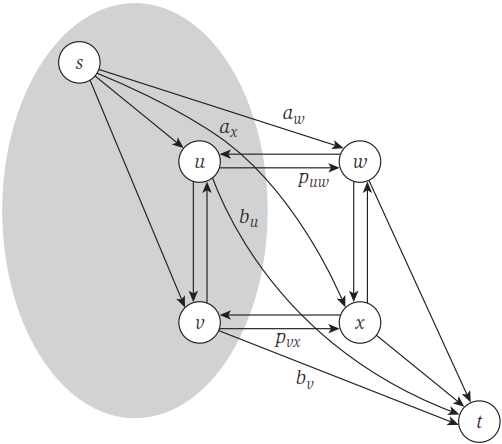
\includegraphics[width=.4\textwidth]{reduction}
	\end{figure}
	\begin{itemize}
		\item Create source $s$ and sink $t$ to represent FG and BG, resp
		\item Attach $s$ and $t$ to every pixel and use $a_i$ and $b_i$ to define edge capacities on $s$, $t$, and each $i$.
		\item Replace undirected edges between each pixel to two directed edges.
		\item<3-> Produces flow network $G' = (V', E')$
	\end{itemize}
\end{frame}

\begin{frame}{Reduction to Max Flow Problem}
	\begin{figure}
		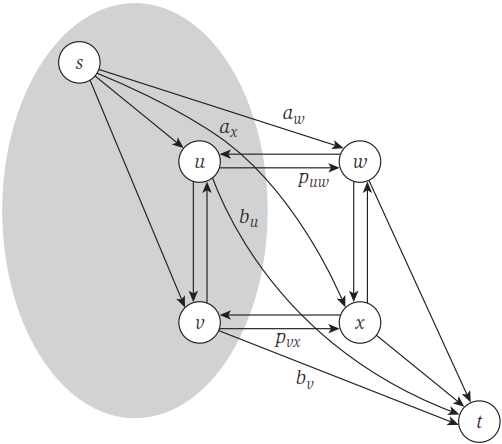
\includegraphics[width=.4\textwidth]{reduction}
	\end{figure}
	Group the edges that cross the cut into three
	\begin{itemize}
		\item Edges $(s, j), j \in B$, contributes $a_j$ to $c(A, B)$
		\item Edges $(i, t), i \in A$, contributes $b_i$ to $c(A, B)$
		\item Edges $(i, j), i \in A, j \in B$, contributes $p_{ij}$ to $c(A, B)$
		\item Adding them all we get $c(A, B) = q'(A, B)$
	\end{itemize}
\end{frame}

\begin{frame}{Reduction to Max Flow Problem}
	\begin{figure}
		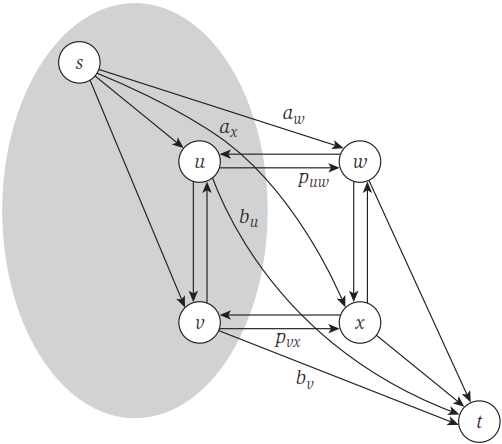
\includegraphics[width=.4\textwidth]{reduction}
	\end{figure}
	$$c(A, B) = \sum_{i \in A} b_i + \sum_{j \in B} a_j + \sum_{\substack{(i, j) \in E \\ \left|A \cap \{i, j\}\right| = 1}}p_{ij} = q'(A, B)$$
	Solution is obtained by a minimum-cut algorithm in the graph $G'$. The partition obtained by deleting $s$ and $t$ maximizes the reward $q(A,B)$.
\end{frame}
	
\section{Local Search}
\subsection{State-Flipping Algorithm}
\begin{frame}{State-Flipping Algorithm}
	Used to obtain neighbors for local searches in graph partitions.
	\begin{block}{State-Flipping Algorithm}
		If there exists a node $u$ s.t. $$\sum_{i\:\in\:\text{edges from}\:u\:\text{into}\:A}w(i) > \sum_{j\:\in\:\text{edges from}\:u\:\text{out of}\:A}w(j)$$
		then $u$ should be moved on the other partition.
	\end{block}
	Two labelings are neighboring solutions if one can be obtained from the other by executing a single node flip.
\end{frame}

\begin{frame}{State-Flipping Algorithm}
	\begin{figure}
		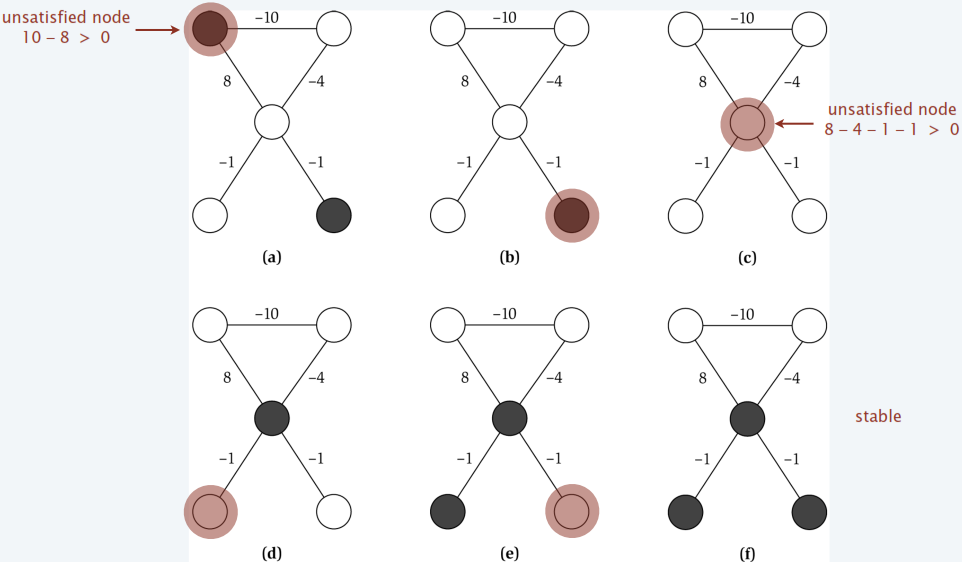
\includegraphics[width=\textwidth]{sfa}
	\end{figure}
\end{frame}

\begin{frame}{Choosing a Neighbor Relation}
	\begin{block}{2-approximation}
		Let $(A, B)$ be a partition that is a local optimum obtained from the single-flip nbhd. Let $(A^*, B^*)$ be a globally optimal partition. Then $$2 \cdot w(A,B) \geq w(A^*, B^*).$$
	\end{block}
	\begin{block}{$k$-flip nbhd, $k > 1$}
		Two labelings are neighbors under the $k$-flip rule if one can be obtained from the other by flipping at most $k$ nodes.
	\end{block}
\end{frame}

\subsection{Classification via Local Search}
\begin{frame}{Classification via Local Search}
	\begin{itemize}
		\item<1-> To obtain good performance, we use an exponentially large nbhd
		\item<1-> But we will need more sophisticated algo to find improving neighbor if it exists.
		\item<2-> Recall the basic ISP. We now consider labeling with more than two labels.
	\end{itemize}
\end{frame}

\begin{frame}{General Labeling Problem}
	Given a graph $G=(V, E)$ and a set of labels $L$. The goal is to label each node to minimize penalty.
	\begin{itemize}
		\item<1-> For each edge $(i, j) \in E$, we have a separation penalty $p_{ij}$ for labeling $i$ and $j$ differently.
		\item<1-> For each node $i \in V$ and each label $a \in L$, we have a penalty $c(i, a) \geq 0$ for assigning label $a$ to node $i$.
	\end{itemize}
	\begin{block}<2->{Labeling Problem}
		Find a labeling $f : V \rightarrow L$ that minimizes the total penalty
		$$\Phi(f) = \sum_{i \in V} c(i, f(i)) + \sum_{\substack{(i, j) \in E\\f(i) \neq f(j)}}p_{ij}$$
	\end{block}
\end{frame}

\begin{frame}{\textit{First Attempt:} the Single-Flip Rule}
	\begin{figure}
		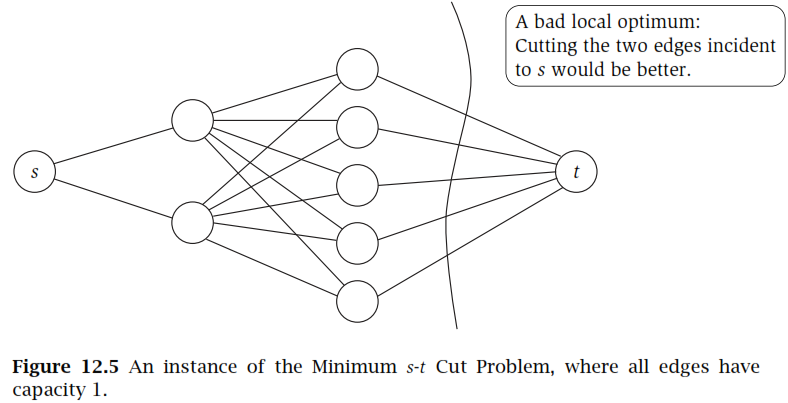
\includegraphics[width=.8\textwidth]{sfr}
	\end{figure}
	\begin{itemize}
		\item<1-> Two labelings are neighbors if one can be obtained from the other by flipping a single node.
		\item<1-> Can lead to quite poor local optima, not a good approx algo for min cut problem
	\end{itemize}
\end{frame}

\begin{frame}{Considering two Labels at a Time}
	\begin{itemize}
		\item We pick two labels $a$ and $b$ in labeling $f$. In a single local step, allow any subset of nodes to flip labels $a \leftrightarrow b$.
		\item Two labelings $f$ and $f'$ are neighbors if there are two labels $a, b \in L$ such that $\forall c \in L \neq a, b, \forall i \in V$ we have $$f(i) = c \Leftrightarrow f'(i) = c$$
		\item Note that $f$ can have exponentially many neighbors, $ \leq 2^x$. However,
	\end{itemize}
	\begin{block}{Theorem 12.8}
		If a labeling $f$ is not locally optimal for the nbhd, a better neighbor can be found via $k^2$ min cut computations. \textit{There are fewer than $k^2$ pairs of distinct labels, $k \mathbf{C} 2$, and we try each pair separately. To find best improved labeling via swapping two labels is exactly SP.}
	\end{block}
\end{frame}

\begin{frame}{Considering two Labels at a Time}
	Solve two labels optimally but local optima can still be bad
	\begin{figure}
		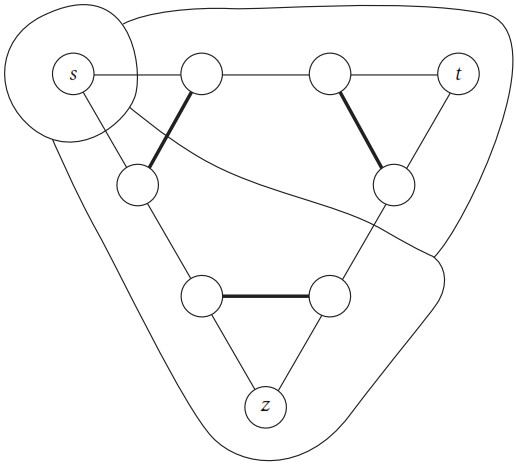
\includegraphics[width=.4\textwidth]{twol}
	\end{figure}
	\begin{itemize}
		\item<1-> Three nodes required to keep their labels
		\item<1-> Other nodes should get one of the labels on the same side of triangle
		\item<1-> Give each node large penalty for labels not allowed
		\item<1-> Light edges have penalty 1, heavy edges have penalty $\infty$
	\end{itemize}
\end{frame}

\begin{frame}{Considering two Labels at a Time}
	Solve two labels optimally but local optima can still be bad
	\begin{figure}
		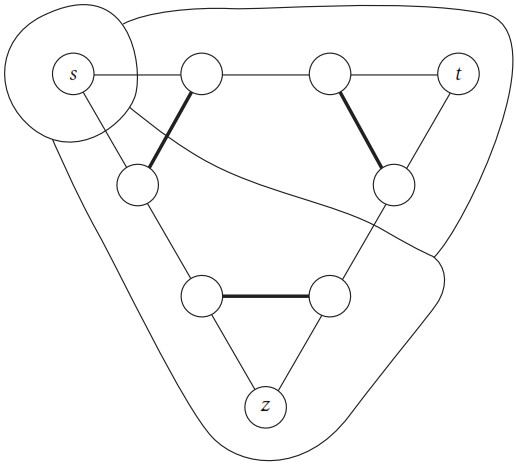
\includegraphics[width=.4\textwidth]{twol}
		\hfil
		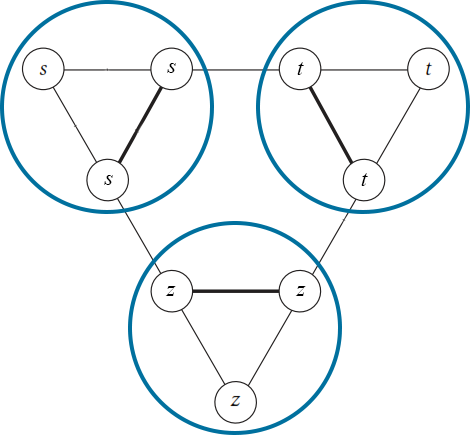
\includegraphics[width=.35\textwidth]{twoopt}
	\end{figure}
	\begin{itemize}
		\item<1-> Light edges have penalty 1, heavy edges have penalty $\infty$
		\item<1-> Current labeling has penalty $M+3$ but locally optimal.
		\item<2-> Global optimal is only $3$
	\end{itemize}
\end{frame}

\begin{frame}{A More Local Search Nbhd that Works}
	\textit{Idea}: Relabel nodes of different labels in a single step
	\begin{itemize}
		\item<1-> Pick one label $a \in L$ and focus on nodes not labeled as $a$
		\item<1-> As a single local step, allow subset of these nodes to change their labels to $a$.
		\item<2-> Two labelings $f$ and $f'$ are neighbors if there is a label $a \in L$ s.t. $\forall i \in V, f'(i) = f(i) \vee f'(i) = a$.
		\item<2-> We can find the best neighbor of $f$ via $k$ min cut computations and a local optimum is a 2-approximation for the labeling problem.
	\end{itemize}
\end{frame}

\begin{frame}{Finding an good neighbor}
	Consider a label $a$.
	\begin{block}{Claim}
		The best relabeling in which nodes may change their labels to $a$ can be found min cut computation.
	\end{block}
	The construction of the network flow $G' = (V', E')$ is analogous to the min cut computation done for two-label ISP.
\end{frame}

\begin{frame}{Finding a good neighbor}
	\begin{figure}
		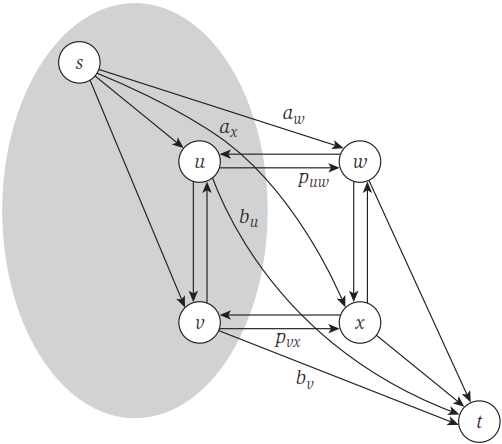
\includegraphics[width=.4\textwidth]{reduction}
	\end{figure}
	\begin{itemize}
		\item Introduce a source $s$ that represent label $a$ and sink $t$ to represent the original labels on the nodes.
		\item Find the min cut in $G'$ and relabel all nodes on the $s$-side to label $a$ while the nodes on the $t$-side will keep their orig labels.
	\end{itemize}
\end{frame}

\begin{frame}{Finding a good neighbor}
	\begin{figure}
		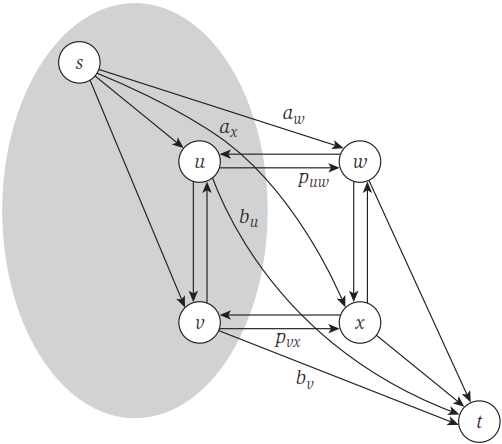
\includegraphics[width=.4\textwidth]{reduction}
	\end{figure}
	\begin{itemize}
		\item Add $G$ to $G'$ as well as edges $(s, i)$ and $(i,t)$ to $E'$.
		\item Edge $(i, t)$ will have capacity $c(i, a)$, as cutting them places node $i$ on the source side and labeling it with $a$.
		\item Edge $(s, i)$ will have capacity $c(i, f(i))$ if $f(i) \neq a$, and $\infty$ if $f(i) = a$ as cutting them places node $i$ on the sink side and retaining its current label.
	\end{itemize}
\end{frame}

\begin{frame}{Finding a good neighbor}
	\begin{figure}
		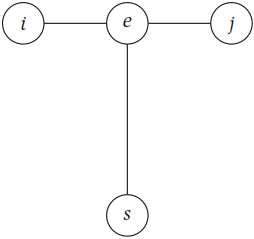
\includegraphics[width=.3\textwidth]{edge}
	\end{figure}
	If both $i$ and $j$ are on the same side, then the edge connecting them is not cut, yet $i$ and $j$ are separated if $f(i) \neq f(j)$.
	\begin{itemize}
		\item For an edge $(i, j)$, if $f(i) = f(j)$ or one if $i$ or $j$ is labeled $a$, then we add an edge $(i, j)$ to $E'$ with capacity $p_{ij}$.
		\item For the rest of the edges, add an extra node  $e$ to $V'$ corresponding to edge $e$, and all the edges $(i,e), (e,j), (e,s)$ with capacity $p_{ij}$.
	\end{itemize}
\end{frame}

\begin{frame}{Finding a good neighbor}
	\begin{block}{Theorem 12.9}
		Given a labeling $f$ and a label $a$, the min cut in the graph $G' = (V', E')$ corresponds to the minimum penalty neighbor of labeling $f$ obtained by relabeling a subset of nodes to label $a$. As a result, a better neighbor can be found via $k$ min cut computations, one for each label in $L$.
	\end{block}
\end{frame}

\begin{frame}{Finding a good neighbor}
	\begin{figure}
		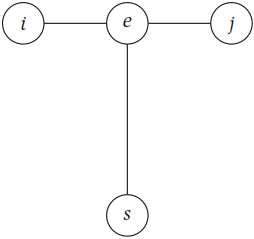
\includegraphics[width=.3\textwidth]{edge}
	\end{figure}
	\begin{itemize}
		\item The large value of $\infty$ ensures that it will not cut heavy edges.
		\item Consider a node $e$ in $G'$ corresponding to an edge $e = (i,j) \in E$. It has three adjacent edges each with capacity $p_{ij}$.
		\item Given any partition, we can place $e$ so that at most one of these edges is cut.
	\end{itemize}
\end{frame}

\begin{frame}{Finding a good neighbor}
	We'll call a cut \textit{good} if 
	\begin{itemize}
		\item<1-> no heavy edge is cut
		\item<1-> for all nodes corresponding to edges in $E$, at most one of the adjacent edges is cut.
	\end{itemize}
	Good cuts in $G'$ are in \textit{one-to-one} correspondence with relabelings of $f$
	\begin{itemize}
		\item<2-> The edges $(s, i)$ and $(i, t)$ contribute exactly the assignment penalty to the capacity of the cut.
		\item<2-> The edges $(i, j)$ contribute exactly the separation penalty
	\end{itemize}
	\begin{block}<3->{Finding a good neighbor}
		As a result, the capacity of a good cut $c(A, B)$ is exactly the same as the penalty of the corresponding labeling $\Phi(f)$, \textit{and so the min cut corresponds to the best relabeling of $f$}.
	\end{block}
\end{frame}

\subsection{Analyzing the Algorithm}
\begin{frame}{Analyzing the Algorithm}
	We'll show that any local optimum under a new neighbor relation is a \textit{2-approximation} to the minimum possible penalty.
	\begin{itemize}
		\item Consider an optimal labeling $f^*$ and for a label $a \in L$, let $V_a^* = \{i : f^*(i)=a\}$ be the set of nodes labeled by $a$ in $f^*$.
		\item Consider a locally optimal labeling $f$. We obtain a neightbor $f_a$ by starting with $f$ and relabeling all nodes in $V_a^*$ to $a$.
		\item Hence, $\Phi(f_a) \geq \Phi(f)$
	\end{itemize}
\end{frame}

\begin{frame}{Analyzing the Algorithm}
	Now, consider the difference $\Phi(f_a) - \Phi(f) \geq 0$. \textit{What quantities contribute to this difference?}
	\begin{itemize}
		\item The change in assignment penalties come from nodes $i \in V_a^*$
		\item The separation penalties differ between the two labelings only in edges $(i, j)$ that have at least one end in $V_a^*$.
	\end{itemize}
	\begin{block}<3->{Theorem 12.10}
		For a labeling $f$ and its neighbor $f_a$, we have
		\begin{align*}
		\Phi(f_a) - \Phi(f) &\leq \sum_{i \in V_a^*} \left[c(i, f^*(i)) - c(i, f(i))\right] \\&+ \sum_{(i, j)\: \text{leaving}\: V_a^*} p_{ij} - \sum_{\substack{(i, j)\: \text{in or leaving}\: V_a^* \\ f(i)\neq f(j)}} p_{ij}
		\end{align*}
	\end{block}
\end{frame}

\begin{frame}{Analyzing the Algorithm}
	\begin{block}{Theorem 12.11}
		For any locally optimal labeling $f$ and any other labeling $f^*$, we have $\Phi(f) \leq 2\Phi(f^*)$. \textit{As a result, all local optima are good approximations to the global optimum.}
	\end{block}
	\textit{Proof}. Since $0 \leq \Phi(f_a) - \Phi(f)$, we have
	\small
	\begin{align*}
	&0 \leq \sum_{a \in L} \left\lbrack \sum_{i \in V_a^*} \left[c(i, f^*(i)) - c(i, f(i))\right] + \sum_{(i, j)\: \text{leaving}\: V_a^*} p_{ij} - \sum_{\substack{(i, j)\: \text{in or leaving}\: V_a^* \\ f(i)\neq f(j)}} p_{ij} \right\rbrack\\
	&\sum_{a \in L} \left\lbrack \sum_{i \in V_a^*} c(i, f^*(i)) + \sum_{(i, j)\: \text{leaving}\: V_a^*} p_{ij} \right\rbrack \geq \sum_{a \in L} \left\lbrack \sum_{i \in V_a^*} c(i, f(i)) + \sum_{\substack{(i, j)\: \text{in or leaving}\: V_a^* \\ f(i)\neq f(j)}} p_{ij} \right\rbrack
	\end{align*}
	\normalsize
\end{frame}

\begin{frame}{Analyzing the Algorithm}
	\begin{itemize}
		\item \textit{left-hand side}: We get $c(i, f^*(i))$ for all nodes $i$, which is exactly the assignment penalty of $f^*$. In addition, we get the term $p_{ij}$ twice for each of the edges separated by $f^*$.
		\item \textit{right-hand side}: We get $c(i, f(i))$ for each node $i$, which is exactly the assignment penalty of $f$. In addition, we get the terms $p_{ij}$ for edges separated by $f$. We get each such separation penalty at least once, and possibly twice if it is also separated by $f^*$.
		\item In summary, we get the following.
		\begin{align*}
		2\Phi(f^*) &\geq \sum_{a \in L} \left\lbrack \sum_{i \in V_a^*} c(i, f^*(i)) + \sum_{(i, j)\: \text{leaving}\: V_a^*} p_{ij} \right\rbrack\\
		&\geq \sum_{a \in L} \left\lbrack \sum_{i \in V_a^*} c(i, f(i)) + \sum_{\substack{(i, j)\: \text{in or leaving}\: V_a^* \\ f(i)\neq f(j)}} p_{ij} \right\rbrack \geq \Phi(f)
		\end{align*}
	\end{itemize}
\end{frame}

\begin{frame}{Analyzing the Algorithm}
	\textit{How fast does the algorithm find a local optimum?} We can only accept big improvements, recall MCP.
	\begin{itemize}
		\item Let $\epsilon > 0$ be a constant.
		\item For a given labeling $f$, we will consider a neighbor $f'$ a \textit{significant improvement} if $\Phi(f') \leq (1-\epsilon/3k) \Phi(f)$
		\item After at most $\epsilon^{-1}k$ significant improvements, the penalty decreases by a constant factor; hence the algorithm will terminate in polynomial time.
	\end{itemize}
\end{frame}

\begin{frame}{Analyzing the Algorithm}
	\begin{block}{Theorem 12.12}
		For any fixed $\epsilon > 0$, the version of the local search algorithm that only accepts significant improvements terminates in polynomial time and results in a labeling $f$ such that $\Phi(f) \leq (2 + \epsilon)\Phi(f^*)$ for any other labeling $f^*$.
	\end{block}
	\textit{Proof.} Since $\epsilon/3k \leq 1$ and $\Phi(f) \leq 2\Phi(f^*)$ from Thm 12.11
	\begin{align*}
	\Phi(f) \leq (2 + \epsilon) \Phi(f^*)
	\end{align*}
	adapting the proof from Thm 12.11.
\end{frame}

\begin{frame}
	\begin{block}{
			\centering
			Thank you for your attention!}
	\end{block}
\end{frame}
\end{document}